% -- Generated using the code: draw_clocks(v1=-0.1, v2=0.4, tstart=-1, tend=7,)
% -- -> moving_clocks_single_fig(-0.1, 0.4, -1, 7, -0.5) is slightly off



% \begin{tikzpicture}
%     % Draw lines of observers
%     \draw[->, thick] (-0.40201512610368484, -0.9547859244962514) -- (-1.2060453783110547, 7.0855165975774455);
%     \draw[->, thick] (0.10910894511799615, -0.8728715609439694) -- (3.600595188893874, 7.855844048495725);
%     \draw[->, thick] (-0.1623618057543558, -1.0130949392667081) -- (1.1365326402804907, 7.091664574866957);

%     % Draw trajectories of light
%     \draw[->, thick, black!10!yellow] (-0.6231234454607115, 1.256297269074015) -- (1.9537009395844693, 3.7386084252222127);
%     \draw[->, thick, black!10!yellow] (1.9537009395844693, 3.7386084252222127) -- (-1.1707397509030126, 6.732460323497025);
%     \draw[->, thick, black!10!yellow] (1.0692676621563626, 1.5275252316519465) -- (-0.8267934763476378, 3.292997577943277);
%     \draw[->, thick, black!10!yellow] (-0.8267934763476378, 3.292997577943277) -- (3.4472811660885947, 7.472558991482527);

%     % Draw lines of simultaneity
%     \draw[thick, blue] (-0.8969315981818621, 3.9943787962855204) -- (2.2582744141224786, 4.500042111567237);
%     \draw[thick, blue] (-0.8267934763476378, 3.292997577943277) -- (1.9537009395844693, 3.7386084252222127);

%     % Make labels
%     \draw (-0.40201512610368484, -0.9547859244962514) node[left] {$\mathcal{O}$};
%     \draw (-0.6231234454607115, 1.256297269074015) node[left] {$t_-$};
%     \draw (-1.1707397509030126, 6.732460323497025) node[left] {$t_+$};
%     \draw (1.9537009395844693, 3.7386084252222127) node[right] {$\tau'$};
%     \draw (2.2582744141224786, 4.500042111567237) node[right] {$t'$};
%     \draw (0.10910894511799615, -0.8728715609439694) node[right] {$\mathcal{O}'$};
%     \draw (1.0692676621563626, 1.5275252316519465) node[right] {$t'_-$};
%     \draw (3.4472811660885947, 7.472558991482527) node[right] {$t'_+$};
%     \draw (-0.8267934763476378, 3.292997577943277) node[left] {$\tau$};
%     \draw (-0.8969315981818621, 3.9943787962855204) node[left] {$t$};
%     \draw (-0.1623618057543558, -1.0130949392667081) node[below] {$\mathcal{R}$};
% \end{tikzpicture}


% -- Generated using moving_clocks(0.1, 0.4, -1, 9, 0.5) from draw_clocks

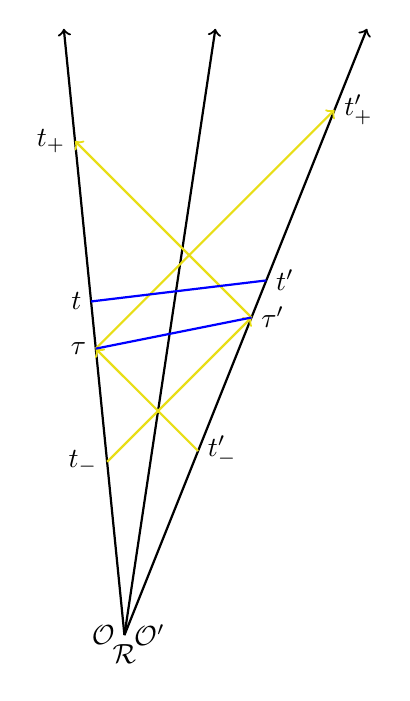
\begin{tikzpicture}[scale=1.1]
	% Draw lines of observers
	\draw[->, thick] (-0.6, -4) -- (-1.3, 3);
	\draw[->, thick] (-0.6000000000000001, -4) -- (2.2, 3);
	\draw[->, thick] (-0.6000000000000001, -4) -- (0.45000000000000007, 3);  % Commenting referee here, is a little deceiving
	
	% Draw trajectories of light
	\draw[->, thick, black!10!yellow] (-0.8, -2) -- (0.8666666666666667, -0.33333333333333326);
	\draw[->, thick, black!10!yellow] (0.8666666666666667, -0.33333333333333326) -- (-1.1703703703703705, 1.703703703703704);
	\draw[->, thick, black!10!yellow] (0.2504201680672269, -1.8739495798319328) -- (-0.930718954248366, -0.6928104575163399);
	\draw[->, thick, black!10!yellow] (-0.930718954248366, -0.6928104575163399) -- (1.8252723311546843, 2.0631808278867103);
	
	% Draw lines of simultaneity
	%\draw[thick, blue] (-1.0018518518518518, 0.0185185185185186) -- (1.1764083411142234, 0.4410208527855588);
	\draw[thick, blue] (-0.9851851851851853, -0.14814814814814803) -- (1.0378462496109555, 0.09461562402738877);
	\draw[thick, blue] (-0.930718954248366, -0.6928104575163399) -- (0.8666666666666667, -0.33333333333333326);
	
	% Make labels
	\draw (-0.6, -4) node[left] {$\mathcal{O}$};
	\draw (-0.8, -2) node[left] {$t_-$};
	\draw (-1.1703703703703705, 1.703703703703704) node[left] {$t_+$};
	\draw (0.8666666666666667, -0.33333333333333326) node[right] {$\tau'$};
	%\draw (1.1764083411142234, 0.4410208527855588) node[right] {$t'$};
	\draw (1.0378462496109555, 0.09461562402738877) node[right] {$t'$};
	\draw (-0.6000000000000001, -4) node[right] {$\mathcal{O}'$};
	\draw (0.2504201680672269, -1.8739495798319328) node[right] {$t'_-$};
	\draw (1.8252723311546841, 2.0631808278867103) node[right] {$t'_+$};
	\draw (-0.930718954248366, -0.6928104575163399) node[left] {$\tau$};
	%\draw (-1.0018518518518518, 0.0185185185185186) node[left] {$t$};
	\draw (-0.9851851851851853, -0.14814814814814803) node[left] {$t$};
	\draw (-0.6000000000000001, -4) node[below] {$\mathcal{R}$};
\end{tikzpicture}